\documentclass{article}
\usepackage[polish]{babel}
\usepackage[T1]{fontenc}
\usepackage{geometry}
\usepackage{chngpage}
\usepackage{graphicx}
\usepackage{subcaption}
\usepackage{algorithm2e}
\usepackage{amsfonts}
\graphicspath{ {./plots/} }
\geometry{margin=2cm}
\usepackage[utf8]{inputenc}
\usepackage{indentfirst}
\usepackage{longtable}
\author{Nie interesuj się}
\title{\vspace{-2.0cm}Sprawozdanie}
\frenchspacing
\setlength{\parindent}{2em}
\begin{document}
\maketitle
\section*{Metoda Bisekcji}
\noindent \textbf{Opis : }\\\\
Naszym celem jest napisanie funkcji rozwiązujacej równanie $f(x) =0$ metodą bisekcji. Metoda bisekcji (połowienia przedziału) korzysta z własności Darboux dla funkcji ciągłej. Oznacza to, że jeśli funkcja $f$ jest ciągła w przedziale ${a,b}$ i zmienia znak ($f(a)*f(b) < 0$) to posiada ona miejsce zerowe w przedziale $(a,b)$.\\\\
Schematyczne działanie algorytmu jest następujące: 
\begin{enumerate}
	\item Jeżeli $f(a)*f(b) < 0$ to obliczane jest $c \leftarrow \frac{a+b}{2}$
	\item Jeżeli $f(a)*f(c) < 0$ to znaczy że f ma zero w $[a,c]$, więc $b \leftarrow c$
	\item W przeciwnym razie jeżeli $f(a)*f(c) < 0$ to znaczy że f ma zero w $[c,b]$, więc $a \leftarrow c$
	\item Powrót do punktu 1.
	\item Program kończy działanie, gdy funkcja nie zmienia znaku (błąd), gdy osiągnięta dokładność jest dostatecznie mała ($|e| < \delta$), lub $f(c)$ jest dostatecznie blisko zera ($|w| < \epsilon$)
\end{enumerate}
W algorytmie pojawia się rówież parę usprawnień:
\begin{enumerate}
	\item Zamiast instrukcji $c \leftarrow \frac{a+b}{2}$ (która w skrajnym przypadku mogłaby nawet 'wypchnąć' punkt $c$ poza przedział $[a,b]$), stosujemy $c \leftarrow \frac{a+b}{2}$ co jest lepsze z numerycznego punktu widzenia.
	\item Zamiast kosztownego mnożenia $f(a)*f(c) < 0$ sprawdzamy zmianę znaku za pomocą funkcji signum
\end{enumerate}
\noindent \textbf{Pseudokod: }\\\\  
\rule{\textwidth}{0.4pt}
\begin{algorithm}[H]
	\KwData{$f,a,b,\delta,\epsilon$}
	\KwResult{$(r,v,it,err)$}
	\vspace{0.3cm}
	$u \leftarrow f(a)$\;
	$v \leftarrow f(b)$\;
	$e \leftarrow b- a$\;
	\If{$sgn(u) = sgn(v)$}
		{\Return{$error (0,0,0,1)$}}
	\While{$true$}{
		$e \leftarrow \frac{e}{2}$\;
		$c \leftarrow a + e$\;
		$w = f(c)$\;
		\If{$|e| < \delta$ or $|w| < \epsilon$}
			{\Return{$(c,w,k,0)$}}
		\eIf{$sgn(w) \neq sgn(u) $}
			{$b \leftarrow c$\; $v \leftarrow w$\;}
			{$a \leftarrow c$\; $u \leftarrow w$\;}
	}
\end{algorithm}
\hrule
\newpage
\section*{Metoda Newtona}
\noindent \textbf{Opis: }\\\\
Celem jest stworzenie funkcji rozwiązującej równanie $f(x)=0$ metodą Newtona. Metoda Newtona, zwana również metodą stycznych, polega na zastąpieniu zadanej funkcji $f$ funkcją liniową. Funkcję liniową tworzą w tym przypadku dwa pierwsze składniki ze zbioru Taylora dla $f$. Metoda ta jest najszybsza z wszystkich używanych teraz przez nas, ponieważ zbieżność jest kwadratowa, lecz nie czyni jej to wcale najlepszą, gdyż nie zawsze jest zbieżna, więc warto łączyć ją z innymi metodami, które są już zbieżne globalnie, w celu osiągnięcia optymalnej szybkości.\\\\
Schematyczne działanie algorytmu jest następujące: 
\begin{enumerate}
	\item Sprawdzany jest warunek początkowy ($f(x0) < \epsilon$), jeżeli zachodzi, to funkcja zwróci błąd.
	\item Dla zadanej liczby iteracji wyznaczane są kolejne przybliżenia zera funkcji, które są dane wzorem rekurencyjnym $x_{n+1} = x_{n} - \frac{f(x_{n})}{f'(x_{n})}$.
	\item Punkt 2 jest powtarzany do momentu aż znalezione zero zmieści się z dokładności, lub odległość kolejnych przybliżeń będzi dostatecznie mała.
	\item Jeżeli powyżesze warunki nie zostaną spełnione, funkcja zwraca błąd, mówiący o nieznalezieniu wyniku dla zadanej liczby iteracji.
\end{enumerate}
\noindent \textbf{Pseudokod: }\\\\ 
\rule{\textwidth}{0.4pt}
\begin{algorithm}[H]
	\KwData{$f,pf,x0,\delta,\epsilon, maxit$}
	\KwResult{$(r,v,it,err)$}
	\vspace{0.3cm}
	$v \leftarrow f(x0)$\;
	\If{$|u| < epsilon$}
	{\Return{$error (x0,v,0,2)$}}
	\For{$k \leftarrow 1$ to $maxit$}{
		$x1 \leftarrow x0 - \frac{v}{pf(x0)}$\;
		$v \leftarrow f(x1)$\;
		\If{$|x1 - x0| < \delta$ or $|v| < \epsilon$}
		{\Return{$(x1,v,k,0)$}}
		$x0 \leftarrow x1$
	}
\end{algorithm}
\hrule
\section*{Metoda Siecznych}
\noindent \textbf{Opis: }\\\\
Celem jest stworzenie funkcji rozwiązującej równanie $f(x) =0$ metodą siecznych. Metoda ta wywodzi się bezpośrednio z metody Newtona i została stworzona by uniknąć wyliczania pochodnej funkcji $f$. W tym celu pochodną $f'(x)$ zastąpiono ilorazem różnicowym $\frac{f(x_{n})-f(x_{n-1})}{x_{n} - x_{n-1}}$. W odróżnieniu od metody Newtona, potrzebny jest jednak dodatkowy punkt początkowy, ponieważ $x_{n+1}$ jest zastąpiony przez $x_{n}$ oraz $x_{n-1}$. Każdy krok w tej metodzie wymaga obliczenia tylko jednej wartości funkcji $f$, co czyni ją, mimo wolniejszej zbieżności od metody Newtona, porównywalnie szybką (Metoda Newtona w każdym kroku oblicza dwie wartości - dla funkcji i pochodnej).\\
Schematyczne działanie algorytmu jest następujące: 
\begin{enumerate}
	\item  Nierówność $|f(x0)| > |f(x1)|$ jest sprawdzana, jeżeli zachodzi, to punkty zamieniane są miejscami.
	\item  Kolejny punkt jest obliczany przy użyciu wzoru rekurencyjnego $x_{n+1} = x_{n} - \frac{f(x_{n})*(x_{n}-x_{n-1})}{f(x_{n}) - f(x_{n-1})}$
	\item Jeżeli osiągnięto pożądaną dokładność, lub odległość między przybliżeniami jest dostatecznie mała, algorytm zwraca wynik. Jeżeli nie, algorytm wraca do punktu pierwszego, lub zwraca błąd jeżeli osiągnięta została maksymalna liczba iteracji. 
\end{enumerate}
\noindent \textbf{Pseudokod: }\\\\  
\rule{\textwidth}{0.4pt}
\begin{algorithm}[H]
	\KwData{$f,x0,x1,\delta,\epsilon, maxit$}
	\KwResult{$(r,v,it,err)$}
	\vspace{0.3cm}
	$fa \leftarrow f(x0)$\;
	$fb \leftarrow f(x1)$\;
	\For{$k \leftarrow 1$ to $maxit$}{
		\If{$|fa| > |fb|$}{
			$x1 \leftrightarrow x0$\;
			$fb \leftrightarrow fa$\;
			}
		$s \leftarrow x0 - \frac{x1 - x0}{fb - fa}$\;
		$x1 \leftarrow x0$\;
		$fb \leftarrow fa$\;
		$x0 \leftarrow x0 - fa*s$\;
		$fa \leftarrow f(x0)$\;
		\If{$|x1 - x0| < \delta$ or $|fa| < \epsilon$}
			{\Return{$(x0,fa,k,0)$}}
	}
	\Return{$(x0,fa,maxit,1)$}
\end{algorithm}
\hrule
\section*{Testy}
Do każdej z zaimplementowanych funkcji napisałem testy jednostkowe, badające poprawność działania metod dla funkcji:
\begin{itemize}
	\item $f(x) = x+4$
	\item $f(x) = x^3 +6*x+9$
	\item $f(x) = x^3 -6*x+9$
\end{itemize}
\section*{Zadanie Czwarte}
\noindent \textbf{Opis: }\\\\
Celem zadania było wyznaczenie pierwiastka równania $sin(x) - \frac{x^{2}}{4} = 0$ przy użyciu każdej z omawianych wcześniej metod.\\\\
\noindent \textbf{Przebieg: }\\\\
Zaimplementowane zostały funkcje:
\begin{itemize}
	\item $sin(x) - \frac{x^{2}}{4}$ - właściwa funkcja badana
	\item $cos(x) - \frac{x}{2}$ - pochodna funkcji właściwej
\end{itemize}
Zastosowane parametry to odpowiednio:
\begin{itemize}
	\item Przedział początkowy dla motody bisekcji - $[a,b]$
	\item Przybliżenie początkowe dla metody Newtona - $x_0 = 1.5$
	\item Przybliżenia początkowe dla metody siecznych - $x_0 = 1.0$ oraz $x_1 = 2.0$
	\item Dokładności pomiarów przyjęte dla wszystkich metod to:
	\begin{enumerate}
		\item $\delta = 0.5 * 10^{-5}$
		\item $\epsilon = 0.5 * 10^{-5}$
		\item $maxit = 50$
	\end{enumerate}
\end{itemize}
\noindent \textbf{Wyniki: }\\\\
\begin{center}
	\begin{tabular}{|p{3cm}|p{3.5cm}|p{4cm}|p{3cm}|p{1,5cm}|} \hline
		\textbf{Metoda} & \textbf{Miejsce Zerowe} & \textbf{Wartość funkcji} & \textbf{Liczba iteracji} & \textbf{Błąd} \\
		\hline
		Bisekcji & $1.9337539672851562$ & $-2.7027680138402843e-7$ & $16$ & $0$ (Brak) \\
		\hline
		Newtona & $1.933753779789742$ & $-2.2423316314856834e-8$ & $4$ & $0$ (Brak) \\
		\hline
		Siecznych & $1.933753644474301$ & $1.564525129449379e-7$ & $4$ & $0$ (Brak) \\
		\hline
	\end{tabular}
\end{center}
\noindent \textbf{Wnioski: }\\\\
Uzyskane wyniki potwierdzają zbieżność każdej z metod w zadanych przedziałach/punktach (zbieżność determinowana przez \textit{współczynnik zbieżności} $a$ każdej z metod). Dla metody bisekcji $a = 1$ - zbieżność jest liniowa, dla metody siecznych $a=\frac{1+\sqrt{5}}{2}$ (nadliniowa), a dla metody Newtona jest to już $a=2$ (kwadratowa). Na podstawie tego może wydawać się, że metoda bisekcji jest metodą najmniej efektywną, jedakże osiągnęła ona wynik najbliższy zadanej dokładności. Niewątpliwą zaletą jest też fakt że jako jedyna jest zbieżna globalnie.
\section*{Zadanie Piąte}
\noindent \textbf{Opis: }\\\\
Celem zadania jest znalezienie wartości zmiennej $x$, dla której przecinają się wykresy funkcji $y=3x$ oraz $y = e^{x}$, używając metody bisekcji i dokładności $\delta = 10^{-4}$ oraz $\epsilon = 10^{-4}$. \\\\
\noindent \textbf{Przebieg: }\\\\
Łatwo zauważyć że aby znależć punkty przecięcia zadanych funkcji, musimy znaleźć rozwiązanie równania: $$e^{x} - 3*x = 0$$\\
Aby łatwo ustalić jakie przedziały dobrać, posłużyłem się graficzną reprezentacją obu tych funkcji:
\begin{figure}[ht]
	\centering
	\begin{subfigure}{.5\textwidth}
		\centering
		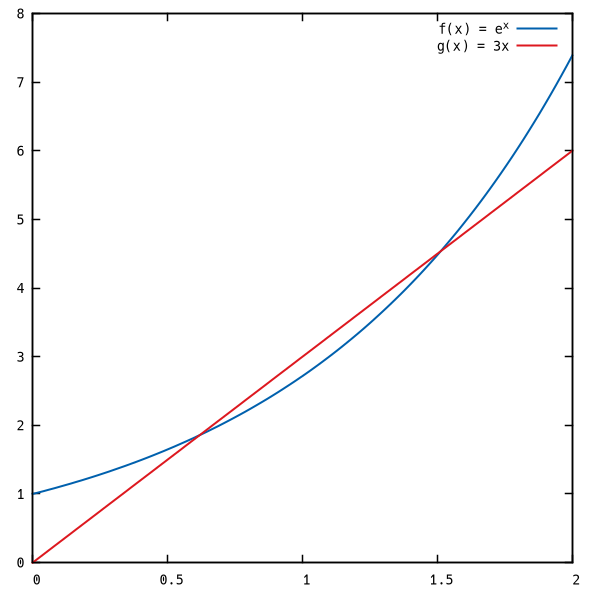
\includegraphics[width=1.0\linewidth]{plots/wykres_1.png}  
		\caption*{Wykres poglądowy, wykonany za pomocą programu GNUplots}
	\end{subfigure}
\end{figure} \\
Jak widać, oba punkty przecięcia znajdują się odpowiednio w przedziałach $[\frac{1}{2},1]$ $[\frac{5}{4},\frac{7}{4}]$
\newpage
\noindent \textbf{Wyniki: }\\\\
\begin{center}
	\begin{tabular}{|p{5cm}|p{5cm}|p{5cm}|} \hline
		 & \textbf{Punkt pierwszy - $x_0$} & \textbf{Punkt drugi - $x_1$} \\
		\hline
		\textbf{Przedział} & $[\frac{1}{2},1]$ & $[\frac{5}{4},\frac{7}{4}]$ \\
		\hline
		\textbf{Wartość} & $0.619140625$ & $1.5120849609375$ \\
		\hline
		\textbf{Niedokładność ($|f(x_i)|$)} & $-9.066320343276146e-5,$ & $7.618578602741621e-5$ \\
		\hline
		\textbf{Liczba iteracji} & $9$ & $12$ \\
		\hline
	\end{tabular}
\end{center}
\noindent \textbf{Wnioski: }\\\\
Podczas użycia metody bisekcji do badania zadanych funkcji, najtrudniejsze okazało się wyznaczenie odpowiednich przedziałów. Można zauważyć że bez pewnych umiejętności analitycznych lub wykresu, ciężko by było wyznaczyć poprawny przedział. Kandydatem mogłoby być np $[0,2]$, na końcach którego funkcja wcale nie zmienia znaku. Na załączony wykresie można łatwo zauważyć jak krótki jest przedział w którym funkcja jest ujemna.
\begin{figure}[ht]
	\centering
	\begin{subfigure}{.5\textwidth}
		\centering
		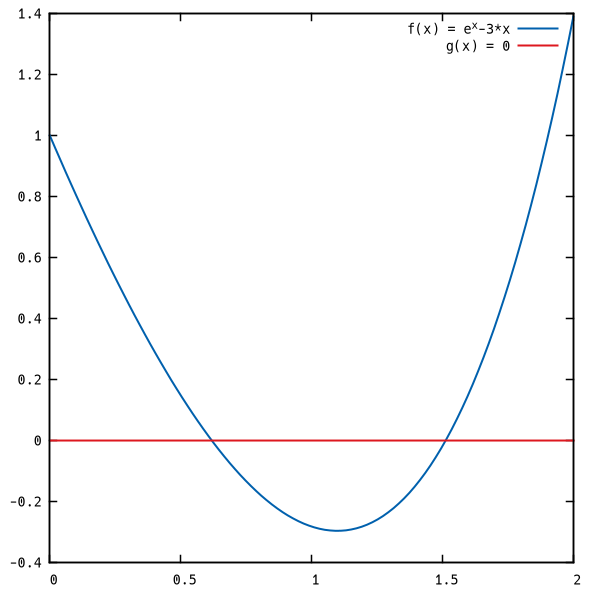
\includegraphics[width=1.0\linewidth]{plots/wykres_2.png}  
	\end{subfigure}
\end{figure} \\
\newpage
\section*{Zadanie Szóste}
\noindent \textbf{Opis: }\\\\
Celem zadania jest znalezienie miejsc zerowych funkcji:
\begin{itemize}
	\item $f_{1}(x) = e^{1-x}-1$
	\item $f_{2}(x) = x*e^{-x}$ 	
\end{itemize}
Przy pomocy zaimplementowanych metod, z zadaną dokładnością obliczeń:
\begin{itemize}
	\item $\delta = 10^{-5}$
	\item $\epsilon = 10^{-5}$
	\item $maxit = 100$
\end{itemize}
\noindent \textbf{Przebieg: }\\\\
\begin{figure}[ht]
	\begin{subfigure}{.5\textwidth}
		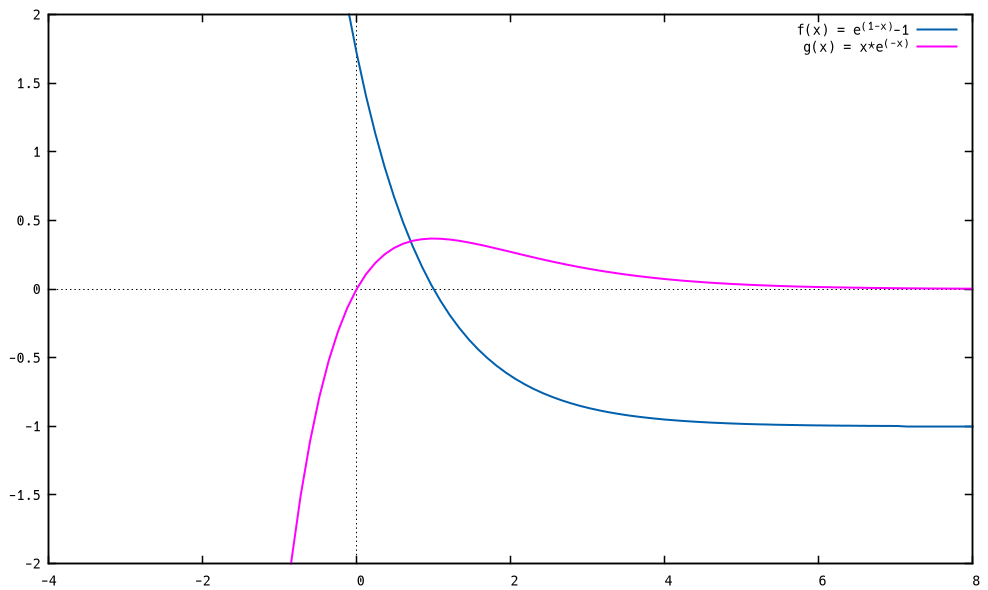
\includegraphics[width=2.0\linewidth]{plots/wykres_3.png}  
	\end{subfigure}
\end{figure} \\
Podczas analizy wykresów zadanych funkcji, od razu nasuwają się poprawne rozwiązania:
\begin{itemize}
	\item $x=-1$ dla $f_{1}(x) = e^{1-x}-1$
	\item $x=0$ dla $f_{2}(x) = x*e^{-x}$ 
\end{itemize}
Z polecenia zadania można jednak wywnioskować że ważniejsze od wyniku jest zbadanie zachowania metod. Wykonałem więc pomiary dla wielu różnych przedziałów i punktów początkowych, aby zbadać wpływ tych danych na wyniki.\\\\
\newpage
\noindent \textbf{Wyniki: }\\\\
Wyniki dla $f_1$ przy użyciu metody bisekcji:
\begin{center}
	\begin{tabular}{|p{3cm}|p{3.5cm}|p{4cm}|p{3cm}|p{2cm}|} \hline
		\textbf{Przedział} & \textbf{Miejsce Zerowe} & \textbf{Wartość funkcji} & \textbf{Liczba iteracji} & \textbf{Błąd} \\
		\hline
		 $[0.0,1.5]$ & $1.0000076293945312$ & $-7.6293654275305656e-6$ & $16$ & $0$  \\
		\hline
		 $[-2.0,4.0]$ & $1.0$ & $0.0$ & $3$ & $0$  \\
		\hline
		 $[0.0,1000.0]$ & $1.0000020265579224$ & $-2.026555868894775e-6$ & $26$ & $0$  \\
		\hline
		 $[-1000.0,1000.0]$ & $1.0000020265579224$ & $-2.026555868894775e-6$ & $27$ & $0$  \\
		\hline
	\end{tabular}
\end{center}
Wyniki dla $f_1$ przy użyciu metody Newtona:
\begin{center}
	\begin{tabular}{|p{3cm}|p{3.5cm}|p{4cm}|p{3cm}|p{2cm}|} \hline
		\textbf{Przybliżenie startowe} & \textbf{Miejsce Zerowe} & \textbf{Wartość funkcji} & \textbf{Liczba iteracji} & \textbf{Błąd} \\
		\hline
		$-1.0$ & $0.9999922654776594$ & $7.734552252003368e-6$ & $5$ & $0$ \\
		\hline
		$0.0$ & $0.9999984358892101$ & $1.5641120130194253e-6$ & $4$ & $0$ \\
		\hline
		$1.0$ & $1.0$ & $0.0$ & $0$ & $2$  \\
		\hline
		$5.0$ & $0.9999996427095682$ & $3.572904956339329e-7$ & $54$ & $0$ \\
		\hline
		$15.0$ & $NaN$ & $NaN$ & $100$ & $1$ \\
		\hline
	\end{tabular}
\end{center}
Wyniki dla $f_1$ przy użyciu metody siecznych:
\begin{center}
	\begin{tabular}{|p{2cm}|p{2cm}|p{3.5cm}|p{4cm}|p{2.5cm}|p{1cm}|} \hline
		\textbf{Przybliżenie startowe 1} & \textbf{Przybliżenie startowe 2} & \textbf{Miejsce Zerowe} & \textbf{Wartość funkcji} & \textbf{Liczba iteracji} & \textbf{Błąd} \\
		\hline
		 $-1.5$ & $2.0$ & $0.9999954314387237$ & $4.568571712271208e-6$ & $7$ & $0$  \\
		\hline
		 $0.0$ & $3.0$ & $0.999999739048799$ & $2.6095123506486573e-7$ & $9$ & $0$  \\
		\hline
		 $-4.0$ & $4.0$ & $3.9487599882268896$ & $-0.9475953519438227$ & $3$ & $0$ \\
		\hline
		 $-5.0$ & $100.0$ & $NaN$ & $NaN$ & $100$ & $1$ \\
		\hline
	\end{tabular}
\end{center}
\vspace{1.0cm}
Wyniki dla $f_2$ przy użyciu metody bisekcji:
\begin{center}
	\begin{tabular}{|p{3cm}|p{3.5cm}|p{4cm}|p{3cm}|p{2cm}|} \hline
		\textbf{Przedział} & \textbf{Miejsce Zerowe} & \textbf{Wartość funkcji} & \textbf{Liczba iteracji} & \textbf{Błąd} \\
		\hline
		$[-0.25,0.5]$ & $7.62939453125e-6$ & $7.62933632381113e-6$ & $15$ & $0$  \\
		\hline
		$[-1.0,4.0]$ & $3.814697265625e-6$ & $3.814682713737527e-6$ & $18$ & $0$ \\
		\hline
		$[-500.0,500.0]$ & $0.0$ & $0.0$ & $1$ & $0$  \\
		\hline
		$[-10.0,1000.0]$ & $495.0$ & $5.234035414371182e-213$ & $1$ & $0$ \\
		\hline
	\end{tabular}
\end{center}
Wyniki dla $f_2$ przy użyciu metody Newtona:
\begin{center}
	\begin{tabular}{|p{3cm}|p{4cm}|p{4cm}|p{3.5cm}|p{1cm}|} \hline
		\textbf{Przybliżenie startowe} & \textbf{Miejsce Zerowe} & \textbf{Wartość funkcji} & \textbf{Liczba iteracji} & \textbf{Błąd} \\
		\hline
		$-2.0$ & $-1.425500682806244e-9$ & $-1.425500684838296e-9$ & $7$ & $0$ \\
		\hline
		$0.0$ & $0.0$ & $0.0$ & $0$ & $2$  \\
		\hline
		$1.0$ & $NaN$ & $NaN$ & $100$ & $1$ \\
		\hline
		$5.0$ & $15.194283983439147$ & $3.827247505782993e-6$ & $9$ & $0$  \\
		\hline
		$15.0$ & $15.0$ & $4.588534807527386e-6$ & $0$ & $2$  \\
		\hline
	\end{tabular}
\end{center}
Wyniki dla $f_2$ przy użyciu metody siecznych:
\begin{center}
	\begin{tabular}{|p{2cm}|p{2cm}|p{3.8cm}|p{4cm}|p{2.5cm}|p{.8cm}|} \hline
		\textbf{Przybliżenie startowe 1} & \textbf{Przybliżenie startowe 2} & \textbf{Miejsce Zerowe} & \textbf{Wartość funkcji} & \textbf{Liczba iteracji} & \textbf{Błąd} \\
		\hline
		$-1.0$ & $1.0$ & $1.744165849924562e-8$ & $1.7441658195034172e-8$ & $18$ & $0$  \\
		\hline
		$0.25$ & $1.5$ & $1.042392303291443e-8$ & $1.0423922924256259e-8$ & $7$ & $0$  \\
		\hline
		$-2.0$ & $5.0$ & $14.699951101212262$ & $6.0702732715516805e-6$ & $13$ & $0$  \\
		\hline
		$-5.0$ & $100.0$ & $100.0$ & $3.7200759760208363e-42$ & $1$ & $0$  \\
		\hline
	\end{tabular}
\end{center}
\noindent \textbf{Wnioski: }\\\\
W przypadku wyników uzyskanych dla metody bisekcji, możemy stwierdzić, że:
\begin{enumerate}
	\item Dla funkcji $f_1$ metoda jest zbieżna do faktycznego punktu zerowego nawet dla dużych przedziałów, jednakże poprzez liniową zbieżność, porzebuje także odpowiednio większej ilości iteracji.
	\item Dla funkcji $f_2$ powinniśmy otrożniej szacować przedział początkowy, poniważ zbiega ona do 0 w nieskończoności, więc przyjęcie zbyt dużego przedziału może zakończyć działanie funkcji już po jednej iteracji (jeden z końców przedziału będzie mniejszy od $\epsilon$)
\end{enumerate}
Dla metody Newtona:
\begin{enumerate}
	\item Dla $f_1$, wraz z oddalaniem się od jedynki w stronę nieskończoności liczba iteracji znacznie rośnie, aż w końcu metoda staje się rozbieżna. Jest to skutkiem stabilizacji funkcji wraz ze zwiększaniem $x$ - skutkiem tego $f(x)$ zaczyna zbiegać do -1, co powoduje zmierzanie pochodnej do zera.
	\item Dla $f_2$, gdy spróbujemy użyć metody Newtona z punktem początkowym $x_0>1$ (pochodna przyjmuje wartość 0 w $x=1$ - maksimum globalne), funkcja przestanie zmierzać do faktycznego zera, lecz znajdzie wartość dostatecznie bliską zera na prawo od punktu 1.
\end{enumerate}
Dla metody siecznych:
\begin{enumerate}
	\item Dla $f_1$ obserwujemy podobne zachowanie jak dla metody Newtona. Jedynym zachowaniem wyróżniającym sie jest przypadek $x_0=-4$ i $x_1=4$, podczas którego w pewnym momencie zadziałał warunek $|x_1-x_0| < \delta$, co spowodowało zakończenie działania metody (analogicznie jak dla $x_0=5$ w metodzie Newtona)
	\item Dla $f_2$ metoda siecznych działa w ten sam sposób jak metoda Newtona.
\end{enumerate}
\end{document}